\documentclass[11pt]{article}

%%%%%%%%%%%%%%%%%%%%%%%%%%%%%%%%%%%%%%%%%%%%%%%%%%%%%%%%
% Imports 		%%%%%%%%%%%%%%%%%%%%%%%%%%%%%%%%%%%%%%%%
%%%%%%%%%%%%%%%%%%%%%%%%%%%%%%%%%%%%%%%%%%%%%%%%%%%%%%%%

	\usepackage{amsmath,amsfonts,amsthm,amssymb,amsopn,bm} %%% load AMS-Latex Package
	\usepackage{graphics,graphicx,subfigure,color} %figures and color	
	\usepackage{mathrsfs}

	%%% paper layout, stylistic etc
	\usepackage{epsfig,fullpage}
	\usepackage{url}
	\usepackage[pdfborder={0 0 1}, colorlinks=true, citecolor=black, plainpages=false]{hyperref}
	\usepackage{parskip} %dont indent paragraphs
	\usepackage[makeroom]{cancel}


	\usepackage{tikz} % graphical models
	\usetikzlibrary{chains,fit,shapes}
	\usetikzlibrary{bayesnet}

%%%%%%%%%%%%%%%%%%%%%%%%%%%%%%%%%%%%%%%%%%%%%%%%%%%%%%%%
% Commands 		%%%%%%%%%%%%%%%%%%%%%%%%%%%%%%%%%%%%%%%%
%%%%%%%%%%%%%%%%%%%%%%%%%%%%%%%%%%%%%%%%%%%%%%%%%%%%%%%%

	\newcommand{\vct}[1]{\boldsymbol{#1}} % vector
	\newcommand{\mat}[1]{\boldsymbol{#1}} % matrix
	\newcommand{\cst}[1]{\mathsf{#1}} % constant
	\newcommand{\T}{^{\textrm T}} % transpose

	\newcommand{\inner}[2]{#1\cdot #2}
	\newcommand{\norm}[1]{\left\|#1\right\|}
	\newcommand{\twonorm}[1]{\|#1\|_2^2}

	\newcommand{\ProbOpr}[1]{\mathbb{#1}} % hollow letter
	\newcommand{\SetOf}[1]{\mathbf{#1}} % Capital set bold letter


	\newcommand{\cind}[3]{{#1} \independent{#2}\,|\,#3}  % conditional independence
	\newcommand{\cndexp}[2]{\ProbOpr{E}\,[ #1\,|\,#2\,]} % conditional expectation

	\newcommand{\degrees}[1]{#1$^{\circ}$} % degrees
	\newcommand{\prob}[1]{\text{p}(#1)} % probability
	\newcommand{\entropy}[1]{\text{H}\left[#1\right]} % entropy
	\newcommand{\expectedValue}[2]{\ProbOpr{E}_{#2}\left(#1\right)} % expected value


	\DeclareMathOperator*{\argmin}{argmin}
	\DeclareMathOperator*{\argmax}{argmax}

	\newcommand{\Eq}[1]{\begin{align*}#1\end{align*}} % conditional expectation

	\newcommand{\italic}[1]{\textit{#1}} % italic
	\newcommand{\boldface}[1]{\textbf{#1}} % bold

	\newcommand{\cursive}[1]{\mathcal{#1}}
	\newcommand{\script}[1]{\mathscr{#1}}

%%%%%%%%%%%%%%%%%%%%%%%%%%%%%%%%%%%%%%%%%%%%%%%%%%%%%%%%
% Document 		%%%%%%%%%%%%%%%%%%%%%%%%%%%%%%%%%%%%%%%%
%%%%%%%%%%%%%%%%%%%%%%%%%%%%%%%%%%%%%%%%%%%%%%%%%%%%%%%%

% \title{PGM Interactive Object Recognition Project}
% \author{Chet Corcos, Karol Hausman, Timmy Mbaya }
\begin{document}

% \maketitle
%\tableofcontents

%\newpage

\section{Notation}
	\begin{itemize}
		\item $N$ objects: $O \in \{o_1,o_2, ..., o_N\}$
		\item $I$ poses: $P \in \{p_1,p_2, ..., p_I\}$
		\item $I$ actions: $A \in \{a_1,a_2, ..., a_I\}$
		\item $K=N\cdot I$ sets of object-poses: $(o_k,p_k) = (o_n,p_i)$
		\item $J$ feature-types: $\SetOf{F} = \{\SetOf{F}^1,\SetOf{F}^2, ..., \SetOf{F}^J\} = \left\{ f_1, ...,  f_M\right\}$
		\item $M_j$ features of type $j$: $\SetOf{F}^j = \{f^j_1,f^j_2, ..., f^j_{M_j}\}$
		\item $R$ traning samples for each object-pose.
	\end{itemize}

\section{Derivation}
	First we record one set of data to build a database:
	% \Eq{\cursive{D} = \left\{ \left(o_k,p_k,\SetOf{F}^1_k, ...,  \SetOf{F}^J_k\right)^{k=K}_{k=1} \right\}}
	\Eq{\cursive{D} = \left\{ \left(o_k,p_k,\SetOf{F}_k\right)^{k=K}_{k=1} \right\}}

	The database is just the set of all unique objects, poses, and features observed in $\cursive{D}$ to create the structure of our Bayesian Network like so:

	\Eq{\SetOf{F} &= \left\{ \SetOf{F}_1, ...,  \SetOf{F}_K\right\} = \left\{ f_1, ...,  f_M\right\}\\
	O &\in \{o_1,o_2, ..., o_N\}\\
	P &\in \{p_1,p_2, ..., p_I\}}


	\begin{center}
	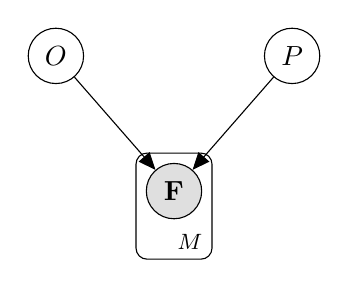
\begin{tikzpicture}
	  % Define nodes
	  \node[obs]                            (F) {$\SetOf{F}$};
	  \node[latent, above=of F, xshift=-1.5cm] (O) {$O$};
	  \node[latent, above=of F, xshift=1.5cm]  (P) {$P$};

	  % Connect the nodes
	  \edge {P,O} {F};

	  % Plates
	  \plate {} {(F)} {$M$}
	\end{tikzpicture}
	\end{center}

	Next, we record a set of training data. For each object-pose, $k$, we record $R$ sets of data:
	\Eq{\cursive{T}_k &= \left\{\left(o^r_k,p^r_k,\SetOf{F}^r_k\right)^{r=R}_{r=1}\right\}\\ \cursive{T} &= \left\{\cursive{T}_1, ..., \cursive{T}_K \right\} }

	An error function must be defined for each feature-type in the model which compares 2 features of the same type:
	\Eq{\cursive{E}^j(\cdot,\cdot)}

	For a training sample $r$, the error with respect to a feature in the model $f^j \in \SetOf{F}$ is the best match with the training features, $\SetOf{F}^r$, defined by:
	\Eq{\cursive{E}_r(f^j) &= \min_{f^j_m \in \SetOf{F}^r}\cursive{E}^j(f^j,f^j_m)}

	We can then learn a distribution of these errors:
	\Eq{\prob{f|o,p} \sim \{\cursive{E}_1(f), ...,  \cursive{E}_R(f)\}}

	After the first observation, we can compute the posterior for all object-poses:
	\Eq{\prob{o,p|\SetOf{F}} &= \frac{\prob{o,p} \cdot \prob{\SetOf{F}|o,p}}{\prob{\SetOf{F}}}\\
	\prob{o,p} &= \frac{1}{K}\\
	\prob{\SetOf{F}|o,p} &= \prod_f \prob{f|o,p}\\
	\prob{\SetOf{F}} &= \frac{1}{K} \sum_{n,i} \prob{\SetOf{F}|o_n,p_i}}

	The next step is to determine the optimal action. After initially observing data $\SetOf{F}_1$, we need to determine the optimal action $a \in A_1$ which will lead to a new pose $P_2$ and reveal new features $\SetOf{F}_2$.
	\begin{center}
	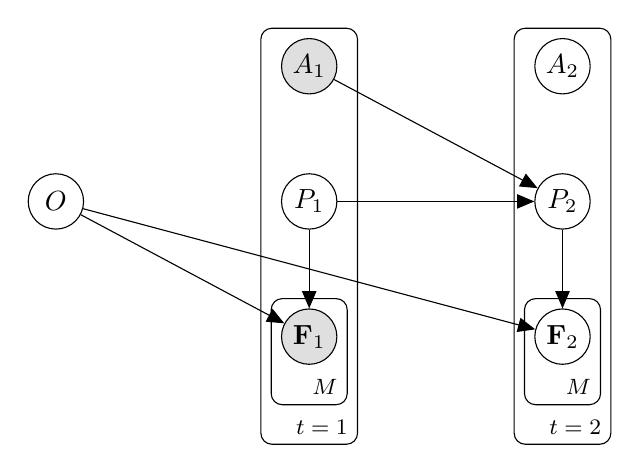
\begin{tikzpicture}
		% Define nodes
		\node[obs] (F) {$\SetOf{F}_1$};
		\node[latent, above=of F]  (P) {$P_1$};
		\node[latent, left=of P, xshift=-1.5cm] (O) {$O$};
		\node[obs, above=of P]  (A) {$A_1$};

		\node[latent, right=of F, xshift=1.5cm] (F2) {$\SetOf{F}_2$};
		\node[latent, above=of F2]  (P2) {$P_2$};
		\node[latent, above=of P2]  (A2) {$A_2$};


	  % Connect the nodes
		\edge {P,O} {F};
		\edge {P2,O} {F2};
		\edge {P,A} {P2};

		% Plates
		\plate {pf} {(F)} {$M$}
		\plate {pf2} {(F2)} {$M$}

		\plate {} {(F)(P)(A)(pf)} {$t=1$}
		\plate {} {(F2)(P2)(A2)(pf2)} {$t=2$}

	\end{tikzpicture}
	\end{center}

	Consider actions as pariwise \italic{relative} actions between poses. For example, an action could be flip upside-down. 
	\Eq{\prob{o,P_2|\SetOf{F}_1,\SetOf{F}_2,a} &= \frac{\sum_{P_1} \prob{o,P_1|\SetOf{F}_1} \; \prob{\SetOf{F}_2|P_2,o} \; \prob{P_2|P_1,a}}{\sum_{P_1,P_2,O} \prob{O,P_1|\SetOf{F}_1} \; \prob{\SetOf{F}_2|P_2,O} \; \prob{P_2|P_1,a}}}

	To determine the optimal action, it we need the probability of the object regardless of pose:
	\Eq{\prob{o|\SetOf{F}_1,\SetOf{F}_2,a} &= \frac{\sum_{P_1,P_2} \prob{o,P_1|\SetOf{F}_1} \; \prob{\SetOf{F}_2|P_2,o} \; \prob{P_2|P_1,a}}{\sum_{P_1,P_2,O} \prob{O,P_1|\SetOf{F}_1} \; \prob{\SetOf{F}_2|P_2,O} \; \prob{P_2|P_1,a}}}

	Note that $\prob{P_2|P_1,A_1} \in \{0,1\}$ is deterministic. Also note that since we have yet to observe $\SetOf{F}_2$, $\prob{\SetOf{F}_2|P_2,o}$ is a joint distribution. Thus $\prob{o|\SetOf{F}_1,\SetOf{F}_2,a}$ is a mixture of joint distributions divided by a mixture of joint distributions.

	Thus, an optimal action would minimize the entropy of \italic{expected} object probabilities.

	\Eq{a^* &= \argmin_{A_1} \entropy{\expectedValue{O|\SetOf{F}_1,\SetOf{F}_2,A_1}{\SetOf{F}_2 \sim \prob{\SetOf{F_2}|\SetOf{F}_1,A_1}}}}

	Now lets generalize to the $n$th action.
	
	\begin{center}
	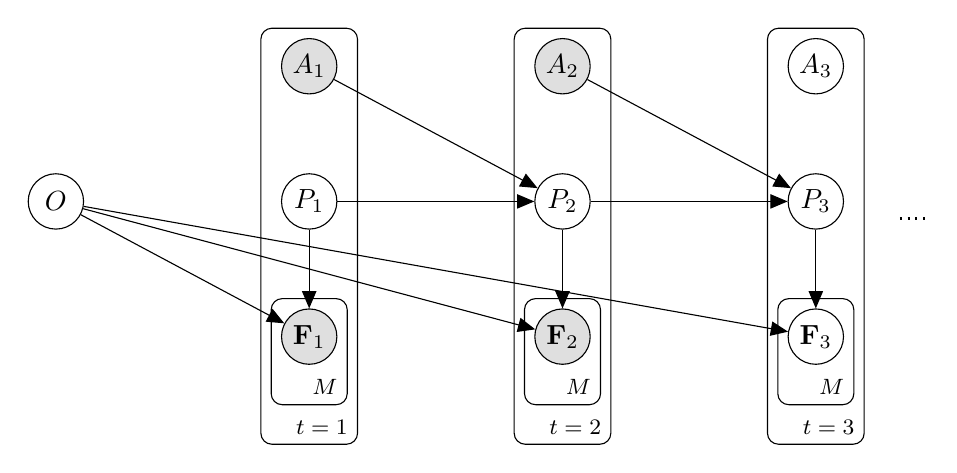
\begin{tikzpicture}
		% Define nodes
		\node[obs] (F) {$\SetOf{F}_1$};
		\node[latent, above=of F]  (P) {$P_1$};
		\node[latent, left=of P, xshift=-1.5cm] (O) {$O$};
		\node[obs, above=of P]  (A) {$A_1$};

		\node[obs, right=of F, xshift=1.5cm] (F2) {$\SetOf{F}_2$};
		\node[latent, above=of F2]  (P2) {$P_2$};
		\node[obs, above=of P2]  (A2) {$A_2$};

		\node[latent, right=of F2, xshift=1.5cm] (F3) {$\SetOf{F}_3$};
		\node[latent, above=of F3]  (P3) {$P_3$};
		\node[latent, above=of P3]  (A3) {$A_3$};


	  % Connect the nodes
		\edge {P,O} {F};
		\edge {P2,O} {F2};
		\edge {P3,O} {F3};
		\edge {P,A} {P2};
		\edge {P2,A2} {P3};

		% Plates

		\plate {pf} {(F)} {$M$}
		\plate {pf2} {(F2)} {$M$}
		\plate {pf3} {(F3)} {$M$}

		\plate {} {(F)(P)(A)(pf)} {$t=1$}
		\plate {} {(F2)(A2)(pf2)} {$t=2$}
		\plate {} {(F3)(A3)(pf3)} {$t=3$}

		\draw [dotted, thick] (7.5,1.5) -- (7.85,1.5);
	\end{tikzpicture}
	\end{center}

	\Eq{\prob{o,P_{n+1}|\SetOf{F}_{1:n+1},A_{1:n}} &= \frac{ \sum_{P_n} \prob{o,P_n|\SetOf{F}_{1:n},A_{1:n-1}} \prob{\SetOf{F}_{n+1}|o,P_{n+1}} \prob{P_{n+1}|P_n,A_n}}{\sum_{P_n,P_{n+1},O} \prob{o,P_n|\SetOf{F}_{1:n},A_{1:n-1}} \prob{\SetOf{F}_{n+1}|o,P_{n+1}} \prob{P_{n+1}|P_n,A_n}} }

	Note that we are merely updating the previous posterior, $\prob{o,P_n|\SetOf{F}_{1:n},A_{1:n-1}}$. 

	\Eq{a^* &= \argmin_{A_n} \entropy{\expectedValue{O|\SetOf{F}_{1:n+1},A_{1:n}}{\SetOf{F}_{n+1} \sim \prob{\SetOf{F_{n+1}}|\SetOf{F}_{1:n},A_{1:n}}}}}

\section{Algorithm}

	From the training, we learn $\prob{f|o,p}$.  
	
	We must keep track of the posterior, evidence, and likelihoods.

	\begin{center}
		\begin{tabular}{c|c|c|c} % number of columns and vertical lines
			\hline % top horizontal line
			Time & Posterior & Evidence & Likelihood\\
			[0.5ex] % [0.5ex] adds vertical space
			\hline\hline % inserts double-line
			0 & $\prob{o,p}$ & & \\[0.5ex] 
			1 & $\prob{o,p|\SetOf{F}_1}$ & $\prob{\SetOf{F}_1}$ & $\prob{\SetOf{F}_1|o,p}$ \\[0.5ex] 
			2 & $\prob{o,p|\SetOf{F}_1,\SetOf{F}_2,A_1}$ & $\prob{\SetOf{F}_2|\SetOf{F}_1,A_1}$ & $\prob{\SetOf{F}_2|o,p}$ \\
			...&...&...&...\\[0.5ex] 
			t & $\prob{o,p|\SetOf{F}_{1:t},A_{1:t-1}}$ & $\prob{\SetOf{F}_t|\SetOf{F}_{1:t-1},A_{1:t-1}}$ & $\prob{\SetOf{F}_t|o,p}$
		\end{tabular}
		\label{tab:reference}
	\end{center}

	We want to keep track of the posterior for each $o,p$. If we observe $\SetOf{F}_t$, then we can directly compute the likelihood 
	\Eq{\prob{\SetOf{F}_t|o,p} &= \prod_{f_t \in \SetOf{F}_t} \prob{f_t|o,p}} 
	and update the posterior
	\Eq{\text{posterior}_t &= \frac{\text{posterior}_{t-1}*\text{likelihood}_t}{\text{evidence}_t}\\
	&= \frac{\text{posterior}_{t-1}*\text{likelihood}_t}{\sum \text{posterior}_{t-1}*\text{likelihood}_t}}

	However, when we predict the optimal action, the likelihood is not observed. This likelihood is a very high dimensional joint distribution. To make computation easier, we can sample the distribution. Because $\prob{\SetOf{F}_t|o,p} = \prod_{f_t \in \SetOf{F}_t} \prob{f_t|o,p}$ is composed of independent features, we can sample from each distribution individually and combine them into a multidimensional sample of the distribution. We can treat these samples as particles. 

	First compute the evidence distribution, 
	\Eq{\prob{\SetOf{F}_{t+1}|\SetOf{F}_{1:t},A_{1:t}} &= \sum_{O,P_{t+1},P_{t}}\prob{O,P_{t}|\SetOf{F}_{1:t},A_{1:t-1}}\prob{\SetOf{F}_{t+1}|O,P_{t+1}}\prob{P_{t+1}|P_t,A_t}}
	Considering actions are deterministic, $A_t*P_t=P_{t+1}$, we can get rid of one of the summations:
	\Eq{\prob{\SetOf{F}_{t+1}|\SetOf{F}_{1:t},A_{1:t}} &= \sum_{O,P_{t}}\prob{O,P_{t}|\SetOf{F}_{1:t},A_{1:t-1}}\prob{\SetOf{F}_{t+1}|O,P_{t+1}}}
	The resulting particles are then used to sample the posterior
	\Eq{\prob{o,P_{t+1}|\SetOf{F}_{1:t+1},A_{1:t}} &= \prob{o,P_t|\SetOf{F}_{1:t},A_{1:t-1}} \prob{\SetOf{F}_{t+1}|o,P_{t+1}}_{\SetOf{F}_{t+1} \sim \prob{\SetOf{F}_{t+1}|\SetOf{F}_{1:t},A_{1:t}}}}
	Then, taking the average of these particles gives us the expected value.


	


\section{Questions}
	1) We never learned about bayesian factor graphs, but it seems that we could learn a multivatiate distribution to directly learn $\prob{\SetOf{F}|o,p}$:

	\Eq{\prob{\SetOf{F}|o,p} \sim \left\{ \begin{array}{c} \cursive{E}_1(f_1), ...,  \cursive{E}_R(f_1)\\ \cursive{E}_1(f_2), ...,  \cursive{E}_R(f_2) \\ ... \\ \cursive{E}_1(f_M), ...,  \cursive{E}_R(f_M) \end{array}\right \}}

	\begin{center}
	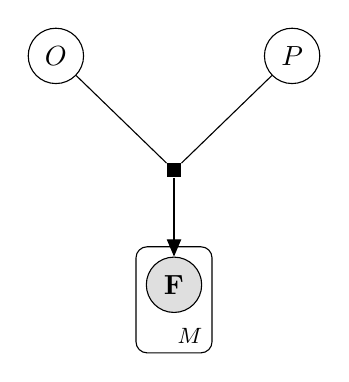
\begin{tikzpicture}
	  % Define nodes
	  \node[factor]                            (f) {};
	  \node[obs, below=of f]                            (F) {$\SetOf{F}$};
	  \node[latent, above=of f, xshift=-1.5cm] (O) {$O$};
	  \node[latent, above=of f, xshift=1.5cm]  (P) {$P$};

	  % Connect the nodes
	  \edge [-] {P,O} {f};
	  \edge {f} {F};

	  % Plates
	  \plate {} {(F)} {$M$}
	\end{tikzpicture}
	\end{center}

	

\section{Appendix}
	\Eq{\prob{\SetOf{F}} &= \sum_{n,i} \prob{o_n,p_i,\SetOf{F}}\\
	&= \sum_{n,i} \prob{\SetOf{F}|o_n,p_i}\cdot \prob{o_n,p_i}\\
	&= \frac{1}{K} \sum_{n,i} \prob{\SetOf{F}|o_n,p_i}}

	\Eq{\prob{o,P_2|\SetOf{F}_1,\SetOf{F}_2,A_1} &= \sum_{P_1} \frac{\prob{o,P_1,P_2,\SetOf{F}_1,\SetOf{F}_2,A_1}}{\prob{\SetOf{F}_1,\SetOf{F}_2,A_1}} \\
	&= \sum_{P_1} \frac{\prob{o,P_1}\prob{A_1}\prob{P_2|P_1,A_1}\prob{\SetOf{F}_1|P_1,o} \prob{\SetOf{F}_2|P_2,o}}{\prob{\SetOf{F}_1,\SetOf{F}_2|A_1}\prob{A_1}} \\
	&= \sum_{P_1} \frac{\prob{o,P_1}\prob{\SetOf{F}_1|P_1,o}}{ \prob{\SetOf{F}_1}} \frac{\prob{\SetOf{F}_2|P_2,o}\prob{P_2|P_1,A_1}}{\prob{\SetOf{F}_2|\SetOf{F}_1,A_1}} \\
	&= \sum_{P_1} \frac{ \prob{o,P_1|\SetOf{F}_1} \prob{\SetOf{F}_2|P_2,o} \prob{P_2|P_1,A_1} }{ \prob{\SetOf{F}_2|\SetOf{F}_1,A_1}} }

	\Eq{\prob{\SetOf{F}_2|\SetOf{F}_1,A_1} &= \sum_{P_1,P_2, O} \frac{\prob{O,P_1, P_2, \SetOf{F}_1, \SetOf{F}_2| A_1}}{\prob{\SetOf{F}_1}} \\ 
	&= \sum_{P_1,P_2, O} \frac{\prob{O,P_1}  \prob{\SetOf{F}_1|O,P_1} \prob{\SetOf{F}_2|O,P_2} \prob{P_2|P_1,A_1}}{\prob{\SetOf{F}_1}} \\ 
	&= \sum_{P_1,P_2, O} \prob{O,P_1|\SetOf{F}_1} \prob{\SetOf{F}_2|O,P_2} \prob{P_2|P_1,A_1}}

	\Eq{\prob{o,P_2|\SetOf{F}_1,\SetOf{F}_2,A_1} &=  \frac{ \sum_{P_1} \prob{o,P_1|\SetOf{F}_1} \prob{\SetOf{F}_2|P_2,o} \prob{P_2|P_1,A_1} }{ \sum_{P_1,P_2, O} \prob{O,P_1|\SetOf{F}_1} \prob{\SetOf{F}_2|O,P_2} \prob{P_2|P_1,A_1}} }

	\Eq{\prob{o|\SetOf{F}_1,\SetOf{F}_2,A_1} &=  \frac{ \sum_{P_1} \prob{o,P_1|\SetOf{F}_1} \prob{\SetOf{F}_2|P_2,o} \prob{P_2|P_1,A_1} }{ \sum_{P_1,P_2, O} \prob{O,P_1|\SetOf{F}_1} \prob{\SetOf{F}_2|O,P_2} \prob{P_2|P_1,A_1}} }

	\Eq{&\prob{o,P_3|\SetOf{F}_1,\SetOf{F}_2,\SetOf{F}_3,A_1,A_2} \\ 
	&= \sum_{P_1,P_2} \frac{\prob{o,P_1,P_2,P_3,\SetOf{F}_1,\SetOf{F}_2,\SetOf{F}_3,A_1,A_2}}{\prob{\SetOf{F}_1,\SetOf{F}_2,\SetOf{F}_3,A_1,A_2}} \\
	&= \sum_{P_1,P_2} \frac{\prob{o,P_1}\prob{A_1}\prob{A_2}\prob{\SetOf{F}_1|o,P_1}\prob{\SetOf{F}_2|o,P_2}\prob{\SetOf{F}_3|o,P_3}\prob{P_2|P_1,A_1}\prob{P_3|P_2,A_2}}{\prob{\SetOf{F}_3|\SetOf{F}_1,\SetOf{F}_2,A_1,A_2} \prob{\SetOf{F}_2|\SetOf{F}_1,A_1} \prob{\SetOf{F}_1} \prob{A_1} \prob{A_2} } \\
	&= \sum_{P_2} \frac{ \prob{o,P_2|\SetOf{F}_1,\SetOf{F}_2,A_1} \prob{\SetOf{F}_3|o,P_3} \prob{P_3|P_2,A_2}}{\prob{\SetOf{F}_3|\SetOf{F}_1,\SetOf{F}_2,A_1,A_2}} }

	\Eq{&\prob{\SetOf{F}_3|\SetOf{F}_1,\SetOf{F}_2,A_1,A_2} \\
	&= \sum_{P_1,P_2,P_3,O} \frac{\prob{o,P_1,P_2,P_3,\SetOf{F}_1,\SetOf{F}_2,\SetOf{F}_3,A_1,A_2}}{\prob{\SetOf{F}_1,\SetOf{F}_2,A_1,A_2}} \\ 
	&= \sum_{P_1,P_2,P_3,O} \frac{\prob{o,P_1}\prob{A_1}\prob{A_2}\prob{\SetOf{F}_1|o,P_1}\prob{\SetOf{F}_2|o,P_2}\prob{\SetOf{F}_3|o,P_3}\prob{P_2|P_1,A_1}\prob{P_3|P_2,A_2}}{ \prob{\SetOf{F}_2|\SetOf{F}_1,A_1} \prob{\SetOf{F}_1} \prob{A_1} \prob{A_2} } \\ 
	&= \sum_{P_2,P_3,O} \prob{o,P_2|\SetOf{F}_1,\SetOf{F}_2,A_1} \prob{\SetOf{F}_3|o,P_3}\prob{P_3|P_2,A_2}  }

	\Eq{\prob{o,P_3|\SetOf{F}_1,\SetOf{F}_2,\SetOf{F}_3,A_1,A_2} &= \frac{ \sum_{P_2} \prob{o,P_2|\SetOf{F}_1,\SetOf{F}_2,A_1} \prob{\SetOf{F}_3|o,P_3} \prob{P_3|P_2,A_2}}{\sum_{P_2,P_3,O} \prob{o,P_2|\SetOf{F}_1,\SetOf{F}_2,A_1} \prob{\SetOf{F}_3|o,P_3}\prob{P_3|P_2,A_2} } }

	\Eq{\prob{o,P_{n+1}|\SetOf{F}_{1:n+1},A_{1:n}} &= \frac{ \sum_{P_n} \prob{o,P_n|\SetOf{F}_{1:n},A_{1:n-1}} \prob{\SetOf{F}_{n+1}|o,P_{n+1}} \prob{P_{n+1}|P_n,A_n}}{\sum_{P_n,P_{n+1},O} \prob{o,P_n|\SetOf{F}_{1:n},A_{1:n-1}} \prob{\SetOf{F}_{n+1}|o,P_{n+1}} \prob{P_{n+1}|P_n,A_n}} }

\end{document}

